%%%%%%%%%%%%%%%%%%%%%%%%%%%%%%%%%%%%%%%%%%%%%%%%%%%%%%%%%%%%%%%%%%%
%% Thermostated particles in one dimension
%% (C) Copyright 1997 by Kenneth Geisshirt (kneth@chem.ruc.dk)
%% Last modified: 30 January 1998
%%%%%%%%%%%%%%%%%%%%%%%%%%%%%%%%%%%%%%%%%%%%%%%%%%%%%%%%%%%%%%%%%%%

\chapter{Controlling the Temperature in One Dimension}
\label{chap:thermostat}

Inelastic collisions were discussed in chapter \ref{chap:Inelas}. In
this chapter we will discuss our results obtained from simulations of
rigid and soft particles undergoing inelastic collisions. The results
presented here are based upon a paper by the author, Paz Padilla,
Eigil L.\ Pr{\ae}stgaard, and S{\o}ren Toxv{\ae}rd \cite{Geisshirt97b}
which is enclosed as appendix \ref{app:D}.

The investigation of the inelastic collisions began by reading a paper
by Du \etal \cite{Du95}. The results presented by Du \etal did seem
very odd, and a desire of understanding emerged. Du \etal find that
when the collisions are inelastic, and even when the particles are
coupled to a thermostatting device, the particles get clamped. One can
easily imagine the clamping when there is no thermostatting device,
and it has been rigorously shown by Haff \cite{Haff83} - see also
chapter \ref{chap:Inelas} for a more detailed discussion on inelastic
collisions. We do not reveal too much of the conclusions of this
chapter by saying that we find that the ``extraordinary'' state found
by Du \etal is an artifact of the model they used.

The simulation cell in one dimension is a line. We have two walls at
$-\frac{L}{2}$ and $\frac{L}{2}$ where $L$ is the length  of the system
(typically $L=1$). One peculiarity of one-dimensional systems is that
no scattering occurs \ie if two particles, $i$ and $j$, initially are
situated so that $x_i > x_j$ then this inequality holds through the
complete simulation.

The rigid particles used in this chapter are all point particles
\ie the radii of the particles are set to zero. Moreover, the mass is
set to $1$. The soft particles interact through the WCA potential, see
Weeks \etal \cite{Weeks71}. The potential is

\begin{equation}
  u(r) = \begin{cases}
    4\epsilon \left[\left(\frac{\sigma}{r}\right)^{12}
      -\left(\frac{\sigma}{r}\right)^{6}\right] + \epsilon 
    & \text{for $r \le \sqrt[6]{2}\sigma$} \\
    0      & \text{otherwise}
  \end{cases}
\end{equation}
where $r$ is the inter-particle separation, $\sigma$ and $\epsilon$
are the Lennard-Jones parameters. The details on how the inelastic
collisions are modelled can be found in section \ref{sect:SoftParticles}.


\section{Semi-closed system}
\label{sect:SemiClosed}
We will analyse a system consisting of $N$ particles
undergoing inelastic collisions. The system is closed in the sense
that no energy flows into the system, while energy is dissipated
through the collisions.

Figure \ref{fig:RigidSemiClosed} shows the granular temperature,
$\mathcal{T} = \frac{1}{N} \sum_{i=1}^N v_i^2$, as function of time. We
see that after a transient period the temperature decays algebraicly. The
slope can easily be found, and we find that Haff's prediction of the
decay is correct.

\begin{figure}
  \begin{center}
    \epsfig{file=Granular/tempsemi.ps,width=7.5cm,height=7.5cm}
  \end{center}
  \caption[The cooling problem]{A
    \protect$\log\protect$-\protect$\log\protect$ plot of 
    the granular temperature as function of time. The number of rigid,
    point particles is 100 and \protect$\epsilon=0.005\protect$. The
    length of the system is
    \protect$1.0\protect$. During the simulation $38467$ collisions
    occurred.\label{fig:RigidSemiClosed}}
\end{figure}

Figures like figure \ref{fig:RigidSemiClosed} can be obtained from
simulations of rigid particles with a radius larger than zero and
various densities. The transient period depends on the density and the
degree of inelasticity. In the case of soft particles the exponent in
Haff's cooling law is not $-2$. The value of the exponent ranges from $-1.16$
to $-1.90$.


\section{Thermostatting devices}
\label{sect:ThermoDevice}
Systems consisting of particles undergoing inelastic collisions
dissipate kinetic energy. This implies that the velocity of the
particles is decreasing as function of time. Obviously we have that
$\mathcal{T} \rightarrow 0$ as $t \rightarrow \infty$. We therefore
have to introduce a thermostatting device in order to control the
temperature in this situation.

Thermostats (as we usually call thermostatting devices) have been used
in Molecular Dynamics simulations for more than two decades. For soft
systems \eg Lennard-Jones particles, the Nos{\'{e}}-Hoover
thermostat (see section \ref{sect:NVTsimul} for details) is a
well-known thermostat. In the case of rigid particles a few attempts
can be found in the literature. In the following we will introduce those
thermostats we have implemented, and present simulations on rigid and
soft particles coupled to the thermostats. In order to check the
functionality of the thermostats we couple them to systems where the
collisions are elastic \ie no energy dissipates. A perfectly working
thermostat is a device that on average ensure that the temperature of
the system is the same as the temperature of the thermostat.

The coupling between the thermostat and the particles is constructed
in the following way: when a particle collides with the left wall, the
velocity of the particle is changed according to the thermostat. 


\subsection{The Gaussian wall}
\label{sect:GaussWall}
The Gaussian wall returns the particles with a new velocity which is
drawn randomly from a Gaussian distribution \ie

\begin{equation}
  P(v) = \frac{m}{k_B T_{\smbox{wall}}} \exp\left(-\frac{mv^2}{2k_B
      T_{\smbox{wall}}}\right) 
\end{equation}
where $T_{\smbox{wall}}$ is the desired temperature. The wall has been
used by Du \etal \cite{Du95}. At first thought this kind of
thermostatting device comes natural since the initial velocity
distribution of the particles is Gaussian, and by choosing velocities
from a Gaussian distribution, one would think that it will preserve
the velocity distribution.

The argument above is not correct which is illustrated by figure
\ref{fig:GaussWall}. The desired temperature of the thermostat,
$T_{\smbox{wall}}$ is set to $1.0$. The temperature of the system
drops quickly to values lower than the thermostat, and the
steady state value is $0.15 \pm 0.05$. If we turn to the soft
particles, we see a similar behaviour. The steady state temperature is
$0.62 \pm 0.02$.

\begin{figure}
  \begin{center}
    \epsfig{file=Granular/gauss.ps,width=7.5cm,height=7.5cm}
  \end{center}
  \caption[The Gaussian wall]{The granular temperature versus the time.
    The system consists of 100 particles and the length of the system is
    1. The left wall is a Gaussian wall.\label{fig:GaussWall}} 
\end{figure}


\subsection{The constant wall}
\label{sect:ConstWall}
The thermostat which we denote the constant wall, is indeed very
simple. When a particle hits the wall, the velocity is always set to
the same value, namely $\sqrt{T_{\smbox{wall}}}$. This corresponds to
the probability distribution

\begin{equation}
  P(v) = 
  \begin{cases}
    1    & \text{for $v = \sqrt{T_{\smbox{wall}}}$} \\
    0    & \text{otherwise}
  \end{cases}
\end{equation}

A thermostatting device like the one described above is very odd seen
from a physical point of view. It has been used by Du \etal \cite{Du95}
and Rapaport \cite{Rapaport92a}. Figure
\ref{fig:ConstWall} shows the granular temperature as it evolves during
a simulation. We see that at first the temperature drops but then recovers,
and at late times it is $T_{\smbox{wall}}$. So far everything
seem to work perfectly. 

\begin{figure}
  \begin{center}
    \epsfig{file=Granular/const.ps,width=7.5cm,height=7.5cm}
  \end{center}
  \caption[The constant wall]{The granular temperature versus the time.
    The system consists of 100 particles and the length of the system is
    1. The left wall is a constant wall.\label{fig:ConstWall}} 
\end{figure}

A correct steady state temperature is not enough to ensure a perfectly
working thermostat - the velocity distribution must be correct as well
which means that it has to be a Maxwell-Boltzmann distribution. The
distribution obtained from the constant wall is \textit{not} a
Maxwell-Boltzmann distribution - only two velocities are possible (for
the rigid particles): $\pm \sqrt{T_{\smbox{wall}}}$. It is not
difficult to understand. When the collisions are elastic
the particles will exchange velocities only. 

For the soft particles the steady state temperature is
incorrect ($0.51 \pm 0.01$), and it is then easy to see that the
constant wall does not work in this case neither.

\subsection{The frequency device}
\label{sect:Freq}
We have implemented yet another thermostat in the following way: at
certain time intervals the velocity of the left-most particle is
changed. The new velocity is chosen randomly from a Gaussian
distribution. The left wall is now a reflecting wall. We have coined
the term frequency thermostat for this implementation. This
thermostatting device has - to our knowledge - never been suggested or
implemented before. 

As indicated by figure \ref{fig:Freq} the frequency thermostat is able
to set the temperature to the correct value ($1.00 \pm
0.13$). Moreover, the velocity distribution is also correct.

\begin{figure}
  \begin{center}
    \epsfig{file=Granular/freq.ps,width=7.5cm,height=7.5cm}
  \end{center}
  \caption[The frequency device]{The granular temperature versus the
    time. The system 
    consists of 100 rigid particles and the length of the system is
    1. The thermostatting device is the so called frequency
    thermostat, and the frequency is $41.15$.\label{fig:Freq}}  
\end{figure}

The frequency thermostat seems to work perfectly for rigid particles
independently of the frequency. This is not true for soft particles; at
high frequencies the thermostat is not able to produce the correct
equilibrium value. The origin of this problem is that equipartition
takes time, and when the kinetic energy of one particle is changed too
often, the system does not have time to relax to equilibrium.

\subsection{The stochastic wall}
\label{sect:StocWall}
If one digs into the literature one finds a very useful thermostatting
device. It is due to Lebowitz \etal \cite{Lebowitz57,Lebowitz78} who
investigated the transport properties of a Knudsen gas and a Lorentz
gas two decades ago but it has been proposed much earlier. Later
Tenenbaum \etal \cite{Tenenbaum82a,Tenenbaum83a} have used it
in MD simulations of Lennard-Jones fluids. Tenenbaum \etal use the
term ``stochastic boundary conditions'' and we adopt it and use
the term ``stochastic wall''.

The velocity of the particle colliding with the walls (in our case the
left wall only) is changed and the new velocity is drawn from the
distribution

\begin{equation}
\label{eq:StocWall}
  P(v) = \frac{vm}{k_B T_{\smbox{wall}}}
     \exp\left({-\frac{mv^2}{2k_B T_{\smbox{wall}}}}\right)
\end{equation}

The thermostatting device described above works perfectly for rigid
and soft particles as figure \ref{fig:StocWall} clearly shows. The
equilibrium temperature is $1.00 \pm 0.14$ for rigid particles and
$0.98 \pm 0.02$ for soft particles.

\begin{figure}
  \begin{center}
    \epsfig{file=Granular/stoc.ps,width=7.5cm,height=7.5cm}
  \end{center}
  \caption[The stochastic wall]{The granular temperature versus the
    time. The system 
    consists of 100 rigid particles and the length of the system is
    1. The thermostat applied is the stochastic wall.\label{fig:StocWall}}  
\end{figure}


\subsection{Nos\'{e}-Hoover}
\label{sect:NHwall}
For more than a decade the Nos\'{e}-Hoover thermostat has been used
frequently; see section \ref{sect:NVTsimul} for details. The
Nos\'{e}-Hoover approach is an extension to the equations of
motion. Similar to the thermostatting device discussed in the
previous sections, we implement a Nos{\'{e}}-Hoover thermostat at the
left wall. The implementation is as follows: instead of the left wall
we have a particle tethered to the point $x_0=-\frac{L}{2}$ by the
potential $u(x) = \half k (x-x_0)^2$ where $x$ is the position of the
particle and $k$ is the force constant. This single particle is
coupled to a Nos\'{e}-Hoover thermostat, and the rest of the particles
are not. Figure \ref{fig:NHwall} shows the temperature as function of
time. 

\begin{figure}
  \begin{center}
    \epsfig{file=Granular/paz.ps,width=7.5cm,height=7.5cm}
  \end{center}
  \caption[The Nos\'{e}-Hoover wall]{The granular temperature versus
    the time. The system 
    consists of 100 soft particles, the length of the system is
    1 and the force constant of the left-most particle is set to 100
    in reduced units. The thermostat applied to the left particle is a
    Nos\'{e}-Hoover thermostat.\label{fig:NHwall}}  
\end{figure}

As figure \ref{fig:NHwall} shows the thermostat sets the temperature
correctly. The equilibrium value of the temperature is $0.99 \pm
0.01$. 

\subsection{Concluding remarks}
As the results reported above show it is important to use a
thermostatting device that actually can control the temperature
correctly. For the rigid particles we see that the stochastic wall as
described in section \ref{sect:StocWall} is the best candidate. For
the soft particles both the stochastic wall and the Nos\'{e}-Hoover
inspired device can be used. For system in higher dimensions than one,
it is easier to implement the stochastic wall for the soft particles.
The use of any other thermostat than the stochastic wall seems to us
to be questionable.

It is not too difficult to understand why the stochastic wall works
well, and why the Gaussian wall does not. Consider a three-dimensional
system: the probability of a particle with velocity $\vec{v}$ arriving
at a wall is \cite{Guggenheim60}

\begin{equation}
\label{eq:WallDistrib}
  P_{\smbox{wall}}(\vec{v}) = \vec{v}\cdot\vec{n}
     f(\vec{v})
\end{equation}
where $\vec{n}$ is a vector normal to the wall, and $f$ is the velocity
distribution which, in equilibrium, is a Maxwell-Boltzmann
distribution. In order to preserve the velocity distribution, the
particles leaving the wall must have the velocities distributed as the
incoming particles, and the thermostat must return the particles
according to equation \eqref{eq:WallDistrib}.


\section{Breakdown of hydrodynamics}
As mentioned in the beginning of the chapter the study of inelastic
colliding particles was inspired heavily by the paper by Du \etal
\cite{Du95}. The main conclusion of Du \etal is that it is possible to
observe a breakdown of hydrodynamics when we try to thermostat
inelastic particles in one dimension. 

The situation in the paper by Du \etal \cite{Du95} is as this: they
simulate $N$ rigid point particles in one dimension. The collisions
are inelastic; typically they set $\epsilon = 0.005$. Moreover, they
have a Gaussian wall at the left wall while the right wall is
reflecting. Independent of the initial positions of the particles an
``extraordinary'' state develops. The ``extraordinary'' state is that
the particles get clamped \ie the particles are to be found at the right
side of the simulation box.

Now the clamping is not a completely unexpected for inelastic
systems. McNamara \etal \cite{McNamara93a, McNamara94a} have
shown numerically that systems (with a thermostatting device) in one
and two dimensions might collapse and Goldhirsch \etal \cite{Goldhirsch93}
have shown that a
clustering instability is possible for dissipative gases. Moreover,
for one-dimensional systems McNamara \etal have shown analytically
that the collapse will occur if
the number of particles exceed a certain threshold; see section
\ref{InelasCollapse} for further details. But for the chosen degree of
inelasticity, Du \etal do not exceed this threshold. Furthermore, Du
\etal report that the clamping does not disappear as $\epsilon
\rightarrow 0$ \ie in the elastic limit. Du \etal refer to the
clamping as the breakdown of hydrodynamics.

We have simulated 100 rigid point particles but instead of the the
Gaussian wall we use the stochastic wall. To measure whether the
particles will get clamped we use the mean position (which in our case is
the same as the centre of mass) \ie we compute $\langle x \rangle =
\frac{1}{N} \sum_{i=1}^N x_i$ during the simulation. Figure
\ref{fig:COM} shows the mean position for simulations with three
different values of $\epsilon$. Figure \ref{fig:COM}a shows the case
of elastic collision, and the mean position fluctuates around zero as
we would expect. The value $\epsilon = 0.005$ is the same value as
chosen by Du \etal \cite{Du95}. The figure indicates a clamping of the
particle, but as we decrease the degree of inelasticity, the clamping
disappears; see figure \ref{fig:COM}c. We strongly believe that the
conclusion by Du \etal is due to an artifact of their thermostat.

\begin{figure}
  \centering
  \mbox{
    \subfigure[$\epsilon=0.0$]{\epsfig{file=Granular/comA.ps,width=4cm}}\quad
    \subfigure[$\epsilon=0.005$]{\epsfig{file=Granular/comB.ps,width=4cm}}\quad
    \subfigure[$\epsilon=10^{-7}$]{\epsfig{file=Granular/comC.ps,width=4cm}}
    }
  \caption[Breakdown of hydrodynamics]{The mean position
    \protect$\langle x \rangle\protect$ versus 
    time. The systems consist of 100 rigid point particles, and the
    left wall is the stochastic wall.}
  \label{fig:COM}
\end{figure}
